\subsection{Statistical properties}
\label{subsec:statistical_properties}
For non-interacting spheres the relation between rotational and translational diffusion coefficient can be obtained \cite{C5SM02754C}. The former is given by the Stokes-Einstein relation
\begin{equation}
	D_{tr} = \frac{k_B T}{6 \pi \eta R}
\end{equation}
and the latter is given by Stokes-Einstein-Debye relation
\begin{equation}
	D_r = \frac{k_B T}{8 \pi \eta R^3}
	,
\end{equation}
where $T$ is the thermostat temperature, $\eta$ the viscosity of the medium and $k_B$ the Boltzmann constant. The relation between $D_{tr}$ and $D_r$ is given by
\begin{equation}
	\frac{D_r}{D_{tr}} = \frac{3}{4 R^2}
	.
\end{equation}
For sufficiently long times, we can estimate the diffusion coefficient as
\begin{equation}
\label{eq:translation_diffusion_vs_displacement}
	D_{tr} = \lim_{\Delta t \to \infty} \frac{1}{6 \Delta t} \langle r^2(\Delta t)\rangle
	,
\end{equation}
where $\langle r^2(\Delta t)\rangle$ is translational mean square displacement (MSD) of particle relatively to its initial position,
\begin{equation}
	\langle r^2(\Delta t)\rangle
	 = \frac{1}{N} \sum_{i=1}^{N} |\boldsymbol{r}_i(t + \Delta t) - \boldsymbol{r}_i(t)|^2
	 .
\end{equation}
Analogously can be defined relation between rotational diffusion coefficient $D_r$ and rotational mean square displacement (RMSD) $\langle \phi^2(\Delta t) \rangle$
\begin{equation}
\label{eq:rotational_diffusion_vs_displacement}
	D_r = \lim_{\Delta t \to \infty} \frac{1}{6 \Delta t} \langle \phi^2(\Delta t)\rangle
	.
\end{equation}
The vector $\Delta u$ of rotational displacement between two particle orientations represented by quaternions $q^{n+1}$ and $q^n$ can be found in the following way. First, we obtain quaternion $\Delta q = q^{n+1}\, q^{n^{-1}}$, where $q^{n^{-1}}$ is the inverse of $q^n$. Then the direction of $\Delta u$ is parallel to the vector part of $\Delta q$ and $|\Delta u|$ equals to the $\cos^{-1}$ of scalar part of $\Delta q$.

When calculating RMSD we have to account for the fact that rotations on angle $
\alpha$ and $\alpha + 2\pi$ are represented by the same unit quaternions. For that we have to accumulate RD over integration steps (separately for every particle). Then the RMSD can be obtained:
\begin{equation}
\label{eq:rotational_mean_square_displacement}
	\langle \phi^2 (\Delta t)\rangle
		= \frac{1}{N} \sum_{i=1}^{N} 
			\left|
				\sum_{j = 0}^{\frac{\Delta t}{\delta t}}
					\Delta\boldsymbol{u}_{i,j}
			\right|^2
	,
\end{equation}
here we break time interval $\Delta t$ into smaller time intervals $\delta t$, which is necessary due to inability to distinguish rotations on angle $\alpha$ and $\alpha + 2\pi$ radians. The accumulation of rotation goes under summation by $j$ index. \textcolor{red}{The $\Delta t$ could be arbitrary big, so I need to sum the rotation over small intervals where particle turns less then $2 \pi$, or calculate the number of $2 \pi$ rotations. The former is simpler to implement. It's integrating over path, but split into small $\Delta t / \delta t$ pieces, on every one of which we can just use $\Delta u$}

The results of test simulation of non-interacting spheres is shown on \figref{fig:diffusion_stats_mean_square_displacement}. As expected, $\langle r^2\rangle$ is proportional to $2 \cdot \tau_{tr} t$, and $\langle \phi_i^2\rangle$ are proportional to $2 \cdot \tau_r t = 2 \cdot (3/10) \tau_{tr} t$. Here $\tau_{tr}$ is translational damping time defined in eq.~\eqref{eq:Translation_damping_time}, and $t$ is simulation time.
\begin{figure}[t]
\centering
	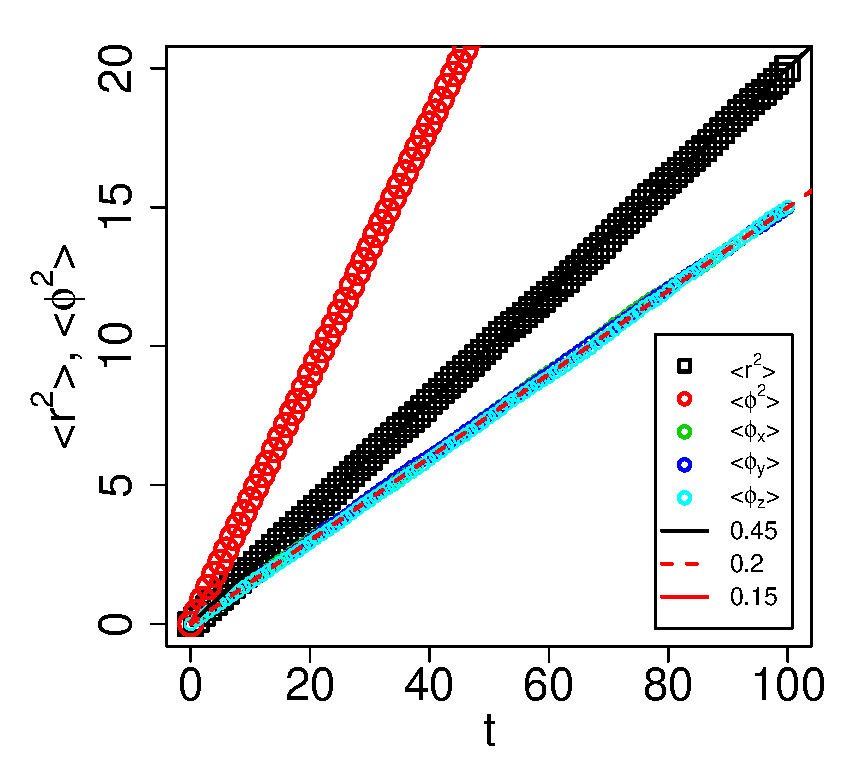
\includegraphics[height=0.7\columnwidth]{Images/DiffusionStats_drift}
%	\captionsetup{justification=justified, width=0.9\columnwidth}
	\caption{Particle MSD and RMSD (with components) as function of time. Points are obtained numerically, with averaging over $20000$ samples. Every sample started from $r_z = v_z = \omega_i = 0$ and particle's  dipole moment co-aligned with $z$ axis. Solid lines are theoretical displacement (eqs. \eqref{eq:translation_diffusion_vs_displacement}, \eqref{eq:rotational_diffusion_vs_displacement}) for given $k_BT = 1$, $m = 1$, $R = 1$ and $\tau_{tr} = 0.1$.}
	\label{fig:diffusion_stats_mean_square_displacement}
\end{figure}
Average kinetic energy per degree of freedom is $1/2 \, k_B T$, which for our case of full three-dimensional rotational and one-dimensional translational movement gives $E_k = 2 k_B T$.

At equilibrium, velocity should satisfy Maxwell-Boltzmann distribution
\begin{equation}
\label{eq:maxwell_boltzmann_velocity}
		p(v^2)
			= \sqrt{ \left(\frac{m}{2 \pi k_B T}\right)^3}
			4 \pi v^2 \exp \left[-\frac{mv_i^2}{2k_BT}\right]
\end{equation}
\begin{equation}
		p(\omega^2)
			= \sqrt{ \left(\frac{I}{2 \pi k_B T}\right)^3}
			4 \pi \omega^2 \exp\left[-\frac{I\omega_i^2}{2 k_B T}\right]
\end{equation}
where $v$ is translational and $\omega$ is rotational velocity, $m$ is particle mass, and $I$ is particle inertia, $k_B$ is Boltzmann constant and $T$ is thermodynamic temperature.

Velocity components should satisfy normal distribution 
\begin{equation}
\label{eq:maxwell_boltzmann_velocity_components}
		p(v_i)
			= \sqrt{ \frac{m}{2 \pi k_BT}}
			\exp \left[-\frac{mv_i^2}{2k_BT}\right]
\end{equation}
\begin{equation}
		p(\omega_i)
			= \sqrt{ \frac{I}{2 \pi k_BT}}
			\exp\left[-\frac{I\omega_i^2}{2k_BT}\right]
\end{equation}
It can be shown that ratio between $\sigma^2_v = k_BT/m$ and $\sigma^2_\omega = k_BT/I$ is
\begin{equation}
\label{eq:velocity_deviation_relation}
	\frac{\sigma^2_v}{\sigma^2_\omega} = \frac{2}{3}R^2
\end{equation}
where $R$ is radius of a particle.

At the \figref{fig:velocity_distributions} the velocity probability distribution are shown, both theoretical and obtained from simulations, for one value of $k_BT = 1$ and $m = 1$. As expected, the $\sigma^2_v / \sigma^2_\omega$ are related as $2/3$ for our case of $R = 1$.
\begin{figure}[t]
\centering
	\begin{minipage}[c]{0.7\columnwidth}
		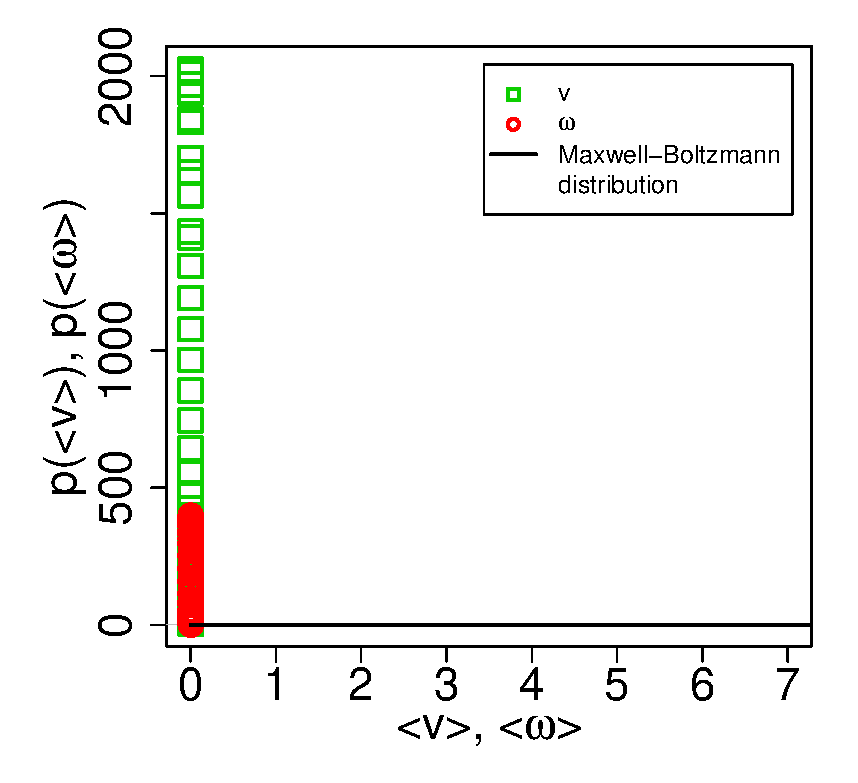
\includegraphics[width=\textwidth]{Images/DiffusionStats_mb}
		\caption{Probability distribution of velocity module. Theoretical distribution is given by equation~\eqref{eq:maxwell_boltzmann_velocity}}
	\end{minipage}
	\begin{minipage}[c]{0.7\columnwidth}
		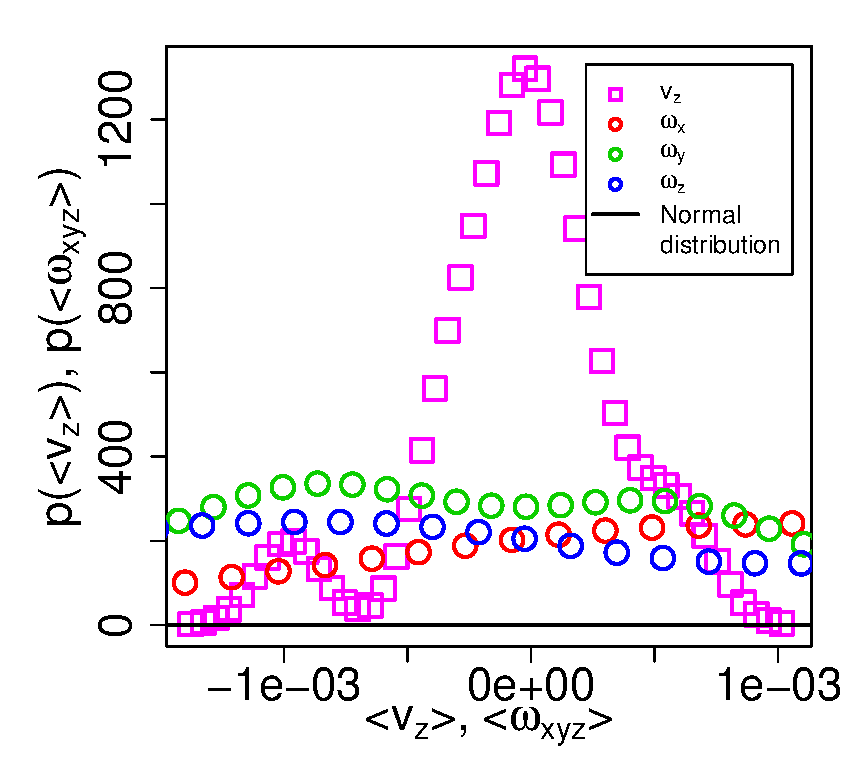
\includegraphics[width=\textwidth]{Images/DiffusionStats_norm}
		\caption{Probability distribution of velocity components. Theoretical distribution is given by equation~\eqref{eq:maxwell_boltzmann_velocity_components}}
	\end{minipage}
	\caption{Translational and rotational velocity probability distribution. Points are obtained numerically, with averaging over $20000$ samples. Every sample started from $r_z = v_z = \omega_i = 0$ and particle's dipole moment co-aligned with $z$ axis. Solid lines are theoretical distributions for given $k_BT = 1$ and $m = 1$.}
	\label{fig:velocity_distributions}
\end{figure}